\documentclass[11pt,a4paper]{article}

% ── Geometry ──────────────────────────────────────────────────────────────────
\usepackage[margin=1in,headheight=14pt]{geometry}

% ── Core packages ─────────────────────────────────────────────────────────────
\usepackage{amsmath,amssymb,amsthm}
\usepackage{mathrsfs}
\usepackage{graphicx}
\usepackage{booktabs}
\usepackage{xcolor}
\usepackage{enumitem}
\usepackage{caption}
\usepackage{subcaption}
\usepackage{needspace}
\usepackage{titlesec}
\usepackage{fancyhdr}
\usepackage{doi}
\usepackage[expansion=false]{microtype}

% ── natbib ────────────────────────────────────────────────────────────────────
\usepackage{natbib}
\setcitestyle{numbers,square,sort&compress}

% ── hyperref (must be near-last) ──────────────────────────────────────────────
\usepackage{hyperref}
\hypersetup{
  colorlinks=true,
  linkcolor=cyan!70!black,
  citecolor=cyan!70!black,
  urlcolor=cyan!70!black,
  pdftitle={TMRB Soft-Hair Resolution of the Black-Hole Information Paradox},
  pdfauthor={George Bressler},
}

% ── Colours ───────────────────────────────────────────────────────────────────
\definecolor{navyblue}{HTML}{0D1B2A}
\definecolor{gold}{HTML}{C8A84B}
\definecolor{cyancol}{HTML}{00B4D8}

% ── Section formatting ────────────────────────────────────────────────────────
\titleformat{\section}
  {\needspace{6\baselineskip}\large\bfseries\color{navyblue}}
  {\thesection}{1em}{}[\color{gold}\titlerule]
\titleformat{\subsection}
  {\needspace{4\baselineskip}\normalsize\bfseries\color{navyblue}}
  {\thesubsection}{1em}{}

% ── Abstract fix (prevent margin bleed) ───────────────────────────────────────
\renewenvironment{abstract}{%
  \begin{quote}\small\textbf{Abstract.}\quad\ignorespaces}%
  {\end{quote}}

% ── Typography ────────────────────────────────────────────────────────────────
\setlength{\emergencystretch}{2em}

% ── Header / Footer ───────────────────────────────────────────────────────────
\pagestyle{fancy}
\fancyhf{}
\fancyhead[L]{\small\color{navyblue}\textbf{BRESSLER 2026 · PTRH PAPER 10 · TMRB SOFT-HAIR BH INFORMATION · ZENODO PREPRINT · CC-BY 4.0}}
\fancyfoot[C]{\small Page \thepage\ · doi:10.5281/zenodo.20326236 · Open access CC-BY 4.0}
\renewcommand{\headrulewidth}{0.4pt}
\renewcommand{\footrulewidth}{0.4pt}

% ── Theorem env ───────────────────────────────────────────────────────────────
\newtheorem{theorem}{Theorem}
\newtheorem{proposition}[theorem]{Proposition}
\newtheorem{conjecture}[theorem]{Conjecture}

% ─────────────────────────────────────────────────────────────────────────────
\begin{document}

% ── Title block ───────────────────────────────────────────────────────────────
\title{%
  \textbf{TMRB Soft-Hair Resolution of the Black-Hole Information Paradox:}\\[4pt]
  \textbf{Discrete $\mathbb{Z}_9$ Torsion Hair, Finite Microstate Counting,}\\[4pt]
  \textbf{and the $9\ln 9$ Topological Correction in 11D M-Theory}%
}
\author{%
  George Bressler\\[2pt]
  ORCID: \href{https://orcid.org/0009-0001-9439-4930}{0009-0001-9439-4930}\\
  \href{mailto:george.bressler@proton.me}{\texttt{george.bressler@proton.me}}\\
  @GeorgeBressler · Sarasota, FL
}
\date{April 2026 (v2: May 2026; v3: May 2026)}
\maketitle
\thispagestyle{fancy}

% ── Prologue ──────────────────────────────────────────────────────────────────
\vspace{4pt}
\begin{center}
{\color{gold}\rule{0.38\textwidth}{0.4pt}}
\end{center}
\vspace{2pt}

\begin{quote}
\itshape
We think of black holes as the universe's ultimate shredders. You fall in,
you are gone, your information destroyed, end of story. Except the laws of
quantum mechanics say information cannot be destroyed --- not as a suggestion,
but as a requirement as fundamental as anything physics has established. So
we have a paradox. The most powerful objects in the universe appear to
violate its most inviolable rule.

Here is where it gets beautiful.

Imagine the surface of a black hole --- the event horizon --- as the world's
most sophisticated recording medium. When you press a vinyl record, the stylus
cuts grooves into the surface: information permanently encoded in the physical
structure of the disc. Every infalling particle, every photon, every quantum of
information that crosses the horizon does the same thing. It cuts a groove. A
gravitational groove. A permanent deformation of the quantum vacuum at the
surface of spacetime itself. Physicists call these imprints \emph{soft hair} ---
because the horizon appears smooth and featureless from the outside, just as
Hawking's equations predict, but at the quantum level it is covered in an
impossibly fine structure that remembers everything that ever fell in.

The question that went unanswered for fifty years is whether that record can
actually be \emph{read}. Hawking's calculation says the radiation emerging from
a black hole is pure thermal noise --- a cosmic hiss carrying no signal, no
memory, no message. The grooves are there, but the record is unplayable.
Information encoded but permanently inaccessible, which is almost worse than
destroyed.

This paper answers that question. The record is not analog. The grooves do not
form a continuous spectrum. The torsion structure of the geometry underlying
the compactification of eleven-dimensional spacetime divides the entire
recording surface into exactly nine orthogonal channels per Planck-area patch
of the horizon. Every possible quantum state that falls into a black hole is
encoded as a chord built from those nine fundamental modes. The radiation coming
out is not noise --- it is the playback, one quantum at a time, through those
same nine channels, in exactly the order the information arrived. The
$\mathbb{Z}_9$ conservation law ensures not a single note is lost.

The universe kept the receipt.

All of this follows from a single observational anchor: one measurement of the
Milky Way's phase spiral by the Gaia satellite, one number,
$\eta_{\mathrm{diff}} = 0.82 \pm 0.02$, which fixes every parameter in the
framework and connects the largest observable structure in our galaxy to the
smallest meaningful scale in physics. That is not a coincidence. That is the
universe telling you something.

What follows is the derivation.
\end{quote}

\vspace{2pt}
\begin{center}
{\color{gold}\rule{0.38\textwidth}{0.4pt}}
\end{center}
\vspace{6pt}

% ── Abstract ──────────────────────────────────────────────────────────────────
\begin{abstract}
The TMRB (Torsion-Modulated Recursive Branching) framework—built on 11D
M-theory compactified on the Schoen gyroid with $\mathbb{Z}_9$ discrete
torsion and golden-ratio modular-covariant branching weights
$w_n = C\exp(-\pi n^2/9)$—has delivered the first discrete holographic dual
for flat spacetime and explicitly closed the infrared triangle linking the
Weinberg soft theorem, BMS supertranslation symmetry, and gravitational memory.
This work completes the UV-to-IR loop by resolving the black-hole information
paradox within the identical construction.

The event horizon carries exactly nine quantised soft-hair charge sectors per
Planck area from the $\mathbb{Z}_9$ gyroid torsion nodes, yielding a finite
horizon Hilbert space of dimension
$\dim\mathcal{H}_{\mathrm{hair}} = 9^{N_{\mathrm{cell}}} = e^{S_{\mathrm{BH}}}$,
where $N_{\mathrm{cell}} = A/(4G_4\ln 9)$ torsion cells tile the horizon.
The Bekenstein--Hawking entropy receives a precise, size-independent topological
correction
\[
  S_{\mathrm{TMRB}} = \frac{A}{4G_4} + 9\ln 9 + \ln 2
    + \mathcal{O}\!\left(\frac{G_4}{A}\right),
  \qquad \Delta S_{\mathrm{tors}} = 9\ln 9 + \ln 2 \approx 20.468,
\]
where $9\ln 9 \approx 19.775$ is the nine-node torsion hair-lattice log-degeneracy
and $\ln 2 \approx 0.693$ is the Euclidean boundary contribution from
$\ln Z_{\rm tors}$.  The golden-ratio weight
$\varphi^{-N_*}$ ($\varphi = (1+\sqrt{5})/2$) exponentially suppresses
logarithmic soft-graviton loop corrections (Section~\ref{sec:loop}), while
holographic unitarity is established by torus partition function factorisation
$Z(\tau)=|\chi_{\mathbb{Z}_9}(\tau)|^2$ (Section~\ref{sec:unitarity}),
together ruling out firewalls and remnants.  All results anchor to the single Gaia DR3
calibration $\eta_{\mathrm{diff}} = 0.82\pm 0.02$.  The 11D CDT extension
invoked here is conjectured; the framework is non-supersymmetric.  Four
correlated near-term falsifiable predictions are presented, together with
quantitative upper limits from coherent narrowband searches of GWOSC O3a
strain data and JPL RL06.3M GRACE-FO mascons that are consistent with --- and
provide a quantitative sensitivity floor for --- the framework's predicted
bulk-gravity-leakage amplitude.

\smallskip
\noindent\textbf{Keywords:} black-hole information paradox, soft hair, BMS symmetry,
torsion, M-theory, CDT, gyroid, holography, Hawking radiation, unitarity.
\end{abstract}

% ── AI Disclosure ─────────────────────────────────────────────────────────────
{\small\textit{AI disclosure: Mathematical iteration via Grok (xAI);
document formatting and refinement via Claude (Anthropic).
All theoretical content, interpretations, and responsibility remain with the author.}}

\vspace{8pt}

% ─────────────────────────────────────────────────────────────────────────────
\needspace{6\baselineskip}
\section{Introduction}
\label{sec:intro}

The black-hole information paradox~\cite{Hawking1975} has resisted resolution for
five decades.  At its core lies a conflict: Hawking's semiclassical calculation
predicts thermal radiation and entropy loss, while unitarity of quantum mechanics
demands that information escaping a black hole remains accessible in principle.
Proposed resolutions range from Planck-scale remnants~\cite{AharonovEtal1987} and
black-hole complementarity~\cite{Susskind1993} to the firewall
conjecture~\cite{AMPS2013} and island-formula approaches~\cite{Penington2020}.

The soft-hair programme of Hawking, Perry, and Strominger
(HPS)~\cite{HawkingPerryStrominger2016} proposed that the horizon carries an
infinite-dimensional memory of soft graviton and soft photon charges, encoding
infalling information.  While compelling, the original proposal left open how the
soft-hair Hilbert space is regularised and how it connects to microscopic string or
quantum-gravity degrees of freedom.

The TMRB (Torsion-Modulated Recursive Branching) framework~\cite{BresslerUF2026,BresslerPrismatic2026}
provides precisely this regularisation.  Compactifying 11D M-theory on the Schoen
gyroid manifold~\cite{Schoen1970} with $\mathbb{Z}_9$ discrete torsion~\cite{BresslerBGL2026}
discretises the Bondi--Metzner--Sachs (BMS) superrotation group to nine generators,
closing the infrared
triangle~\cite{BresslerCH2026} via Weinberg's soft theorem~\cite{Weinberg1965},
BMS supertranslations~\cite{BMS1962,Strominger2014}, and gravitational
memory~\cite{Christodoulou1991,BresslerGP2026}.  The same 3-6-9 torsion
mathematics that sets the 230~Myr galactic disk-wave period and the $\mathbb{Z}_9$
parafermion spectrum at null infinity~\cite{GepnerQiu1987,ZamoFateev1987} now
threads the black-hole event horizon.

This paper demonstrates that:
\begin{enumerate}[leftmargin=*, label=\arabic*.]
  \item The horizon carries exactly \emph{nine} quantised soft-hair charge sectors
    per Planck area from the $\mathbb{Z}_9$ torsion nodes (Section~\ref{sec:hair}).
  \item The Bekenstein--Hawking entropy acquires a universal, size-independent
    torsion correction $\Delta S_{\mathrm{tors}} = 9\ln 9 + \ln 2 \approx 20.468$
    (Section~\ref{sec:entropy}).
  \item Golden-ratio branching weights $w_n = C\exp(-\pi n^2/9)$ exponentially
    suppress logarithmic soft-graviton loop corrections
    (Section~\ref{sec:loop}).
  \item The torus partition function factorises in the discrete holomorphic sector,
    confirming holographic consistency (Section~\ref{sec:unitarity}).
\end{enumerate}

Open theoretical gaps are documented in Section~\ref{sec:gaps}.
Four falsifiable predictions and current observational constraints are
presented in Section~\ref{sec:predictions}.
For the complete series cross-citation map, master parameter table, and
TRL-3/4 test protocol spanning all eight active papers, see~\cite{BresslerSurvey2026}.

\smallskip
\noindent\textbf{Changes in v2:}
\textit{(i)}~BMS spelled out as Bondi--Metzner--Sachs (BMS) on first body use.
\textit{(ii)}~CDT spelled out as Causal Dynamical Triangulations (CDT) on first body use, with explicit AJL citations at definition point.
\textit{(iii)}~$\Delta\lambda$ corrected to 1.7287 (from 1.729) throughout, consistent with all companion papers.
\textit{(iv)}~$Z_{\rm tors} \approx 2$ (not exactly~2; numerical deviation ${\approx}3\times10^{-4}$) corrected at two points.
\textit{(v)}~All cross-citation DOIs updated to canonical versions: TMRB Unified Framework $\to$ v3 (20248650), Celestial Holography $\to$ v4 (20249096), M-Theory Bulk Gravity Leakage $\to$ v10a (20276554), Galactic Piano $\to$ v4 (20262175), QGGPf Predictions $\to$ v4 (20272654).
\textit{(vi)}~Paper~1 (prismatic curvature foundation,~\href{https://doi.org/10.5281/zenodo.20146627}{20146627}) and Paper~9 (PTRH survey,~\href{https://doi.org/10.5281/zenodo.20315669}{20315669}) added to cross-citations.
\textit{(vii)}~\texttt{Vafa1994} bibitem key corrected to \texttt{Vafa1986} (paper is Nucl.~Phys.~B 1986).
\textit{(viii)}~NTRS URL added to Schoen (1970) reference.
\textit{(ix)}~Equation references standardised to \texttt{Eq.\textasciitilde\textbackslash eqref\{\}} throughout.
\textit{(x)}~Footer DOI set to 10.5281/zenodo.19981841.
\textit{(xi)}~\texttt{microtype[expansion=false]} added; \texttt{emergencystretch} corrected to 2em.
\textit{(xii)}~Gap~8 added: derivation of $G_4 = \ell_{\rm Pl}^2/\ln 9$ from the prismatic action is an open item (highest-priority tractable gap in PTRH programme).
\textit{(xiii)}~Gap~9 added: pre-Page-time retrieval protocol remains open.

\smallskip
\noindent\textbf{Changes in v3:}
\textit{(i)}~Horizon Hilbert space formula corrected for Bekenstein consistency:
$\dim\mathcal{H}_{\mathrm{hair}} = 9^{A/(4\ell_{\mathrm{Pl}}^2)}$ (v1/v2) replaced by
$\dim\mathcal{H}_{\mathrm{hair}} = 9^{N_{\mathrm{cell}}} = e^{S_{\mathrm{BH}}}$,
$N_{\mathrm{cell}} = A/(4G_4\ln 9)$ throughout (abstract, \S\ref{sec:microstate},
conclusions); the v1/v2 form exceeds the Bekenstein--Hawking bound by a factor
of $\ln 9 \approx 2.197$ unless the identification $G_4 = \ell_{\mathrm{Pl}}^2/\ln 9$
(Gap~8) is assumed, which is noted explicitly.
\textit{(ii)}~Dangling cross-reference \texttt{app:microstate} removed; the
relevant argument is now inline at Eq.~\eqref{eq:N_hair}.
\textit{(iii)}~All cross-citation DOIs updated to concept DOIs (always resolve
to latest version) throughout.

% ─────────────────────────────────────────────────────────────────────────────
\needspace{6\baselineskip}
\section{TMRB Framework Recap}
\label{sec:recap}

\subsection{Canonical Parameters}

All TMRB results are anchored to a single calibration from Gaia DR3~\cite{GaiaDR3}:
\begin{equation}
  \eta_{\mathrm{diff}} = 0.82 \pm 0.02.
  \label{eq:etadiff}
\end{equation}
The remaining parameters are derived or independently motivated (Table~\ref{tab:params}).

\begin{table}[ht]
\centering
\caption{TMRB canonical parameters. $\kappa_{\mathrm{CE}}$ and $\kappa_{\mathrm{prop}}$
are \emph{distinct} quantities; the former governs conformal-weight combs and
galactoseismology, the latter governs plasma torsion suppression and IAW lock.}
\label{tab:params}
\begin{tabular}{llp{4.0cm}l}
\toprule
Symbol & Value & Role & Domain \\
\midrule
$\eta_{\mathrm{diff}}$ & $0.82\pm0.02$ & Phase-space diffusion ratio & All papers \\
$\lambda_{\mathrm{rec}}$ & 5.2 & Recursive branching depth & All papers \\
$\mu$ & 2.1 & Branching modulation & All papers \\
$\kappa_{\mathrm{CE}}$ & $\mu/\lambda_{\mathrm{rec}} = 0.4038$ & Conformal-weight comb & Holography, galactoseismology \\
$\kappa_{\mathrm{prop}}$ & 0.48 & Torsion suppression exponent & Plasma sector, QGGPf \\
$d_{\mathrm{opt}}$ & 9 & Self-tuned branching depth & All papers \\
$\varphi$ & $(1+\sqrt{5})/2$ & Golden ratio & Branching weights \\
$G_4/G_{11}$ & $(5.214\pm0.12)\times10^{-40}$ & KK hierarchy ratio & Holography, QGGPf \\
$T_0$ & 230~Myr & Galactic disk-wave crest period & Galactoseismology \\
$\eta_{\mathrm{null}}$ & $1.0\pm0.15$ & Null model baseline & All falsification tests \\
\bottomrule
\end{tabular}
\end{table}

\subsection{Gyroid Compactification and $\mathbb{Z}_9$ Torsion}

M-theory is compactified on the Schoen gyroid, a triply-periodic minimal surface
with crystallographic space group $\Gamma = Ia\bar{3}d$ (No.~230)~\cite{Schoen1970}.
The gyroid has no G$_2$ holonomy; the construction is explicitly
non-supersymmetric, with UV finiteness arising from the causal structure of the
conjectured 11D Causal Dynamical Triangulations (CDT) extension~\cite{AJL2004,AJL2005}.

The discrete torsion phases are
\begin{equation}
  \theta_n = \frac{2\pi n}{9}, \qquad n = 0,1,\ldots,8,
  \label{eq:torsion_phases}
\end{equation}
arising from $H^3(\mathbb{Z}_9, U(1)) \cong \mathbb{Z}_9$~\cite{Vafa1986,AspinwallMorrison1995}.  The modular-covariant
branching weights are
\begin{equation}
  w_n = C\exp\!\left(-\frac{\pi n^2}{9}\right),
  \label{eq:wn}
\end{equation}
a \emph{DFT fixed-point Gaussian}: the discrete $\mathbb{Z}_9$ Fourier transform
of $\{w_n\}_{n=0}^{8}$ reproduces the same functional form up to normalisation
(it is a Jacobi theta function $\vartheta_3(0\,|\,i/9)$ evaluated on the
$\mathbb{Z}_9$ lattice), ensuring self-consistency under the modular
$S$-transformation $\tau\to-1/\tau$.  This property replaces the earlier
$\varphi^{-\lambda n}$ form, which lacked modular covariance.
The resulting torsion partition function and associated quantities are:
\begin{align}
  Z_{\mathrm{tors}} &= \sum_{n=0}^{8} \exp\!\left(-\frac{\pi n^2}{9}\right) = \frac{1}{C} \approx 2
    \quad \bigl(\text{deviation from 2 is }{\approx}3\times10^{-4}\bigr),
  \label{eq:Z_tors_val}\\
  \mathcal{S}_{\mathrm{tors}} &= -\sum_{n=0}^{8} w_n \ln w_n \approx 1.068,
  \label{eq:torsion_entropy}\\
  \mathcal{H}_{\mathrm{hair}} &\equiv \ln(9^9) = 9\ln 9 \approx 19.775.
  \label{eq:H_hair}
\end{align}
Here $\mathcal{S}_{\mathrm{tors}}$ is the Shannon entropy of the Gaussian weight
distribution; $\mathcal{H}_{\mathrm{hair}} = 9\ln 9$ is the log-degeneracy of
the full nine-node torsion hair lattice (the number of distinct $\mathbb{Z}_9$
configurations across all nine nodes), equal to $\ln(9^9)$; and
$\ln Z_{\mathrm{tors}} = \ln 2$ is the boundary contribution to the gravitational
path integral.  These three quantities are distinct and are not conflated in what
follows.

\subsection{TMRB Partition Function}

The full partition function is
\begin{equation}
  Z = \sum_{\{\Delta\}} \prod_{\mathrm{links}} e^{i\theta_n}
      \prod_{\mathrm{vertices}} A_{\mathrm{EPRL/FK}}
      \prod_{\mathrm{branches}} w_n,
  \label{eq:Z}
\end{equation}
where $A_{\mathrm{EPRL/FK}}$ are the EPRL/FK spin-foam vertex amplitudes and the
sum runs over all causal dynamical triangulations $\{\Delta\}$ consistent with the
causal structure (11D CDT extension conjectured).

% ─────────────────────────────────────────────────────────────────────────────
\needspace{6\baselineskip}
\section{$\mathbb{Z}_9$ Soft Hair on the Event Horizon}
\label{sec:hair}

\subsection{BMS Superrotations Discretised to $\mathbb{Z}_9$}

In the existing Celestial Holography paper~\cite{BresslerCH2026}, the nine torsion
nodes discretise the BMS superrotation group at null infinity $\mathscr{I}^+$ to
nine generators.  The same mechanism operates at the horizon, which shares the
BMS symmetry structure under Rindler expansion~\cite{Donnay2016}: the near-horizon
geometry in Rindler coordinates $(\rho, t, x^i)$ admits supertranslation charges
$T(z,\bar{z})$ and superrotation charges $Y^z(z)$ on the bifurcation 2-sphere.
The $\mathbb{Z}_9$ torsion phases $\theta_n$ inherited from the bulk
compactification label nine independent charge sectors on the bifurcation surface
by the following argument: the 11D C-field flux restricted to any 3-cycle
$\Sigma_3$ threading the horizon carries the phase $e^{i\theta_n}$; upon
dimensional reduction, this phase labels distinct boundary states on the
bifurcation $S^2$ exactly as at $\mathscr{I}^+$.  This identification follows
directly from the Kaluza--Klein reduction of the 11D C-field on the gyroid:
the discrete torsion classes in $H^3(\mathbb{Z}_9, U(1)) \cong \mathbb{Z}_9$
~\cite{Vafa1986,AspinwallMorrison1995} are preserved by the reduction and project
onto the bifurcation $S^2$ as $\mathbb{Z}_9$-valued boundary phases, mirroring
the discretisation at $\mathscr{I}^+$ established in~\cite{BresslerCH2026}.
Verification that the gyroid reduction preserves this discrete torsion
structure under all moduli of the full 7D internal manifold is an open
technical item (see gap~7 in Section~\ref{sec:gaps}); subject to that
verification, the horizon carries the same discrete BMS dictionary as
$\mathscr{I}^+$.

Each torsion node $n$ carries a conserved soft-hair charge
\begin{equation}
  Q_{\mathrm{super}}^{(n)} = \eta_{\mathrm{diff}} \cdot \theta_n \cdot M_{\mathrm{Pl,11}}^3,
  \label{eq:Q_super}
\end{equation}
where $M_{\mathrm{Pl,11}}$ is the 11D Planck mass, $\theta_n = 2\pi n/9$ is
dimensionless, and $\eta_{\mathrm{diff}}$ anchors the charge normalisation to
the Gaia DR3 calibration.  The charges $Q^{(n)}$ carry dimensions of
$[\text{mass}]^3$ in natural units (equivalently, $[\text{length}]^{-3}$ with
$\hbar = c = 1$); this is the natural dimension of BMS supertranslation charges
in 11D — specifically the stress-energy flux integrated over the bifurcation
2-sphere times the 7D gyroid volume $V_7$, which upon dimensional reduction
gives $Q^{(n)} \sim M_{\mathrm{Pl,4}}$ after absorbing factors of $G_4/G_{11}$.
The numerical coefficient is fixed by requiring that $Q^{(n=1)}$ equals the
minimal KK mass scale set by the gyroid compactification.
The $n=0$ sector has $\theta_0 = 0$ and therefore $Q^{(0)} = 0$; it is the
\emph{vacuum sector} carrying no torsion charge but occupying one of the nine
orthogonal subspaces of the horizon Hilbert space.  The eight sectors
$n=1,\ldots,8$ carry distinct non-zero charges, with $n=9-k$ and $n=k$ related
by $\mathbb{Z}_9$ conjugation.

\begin{figure}[ht!]
\centering
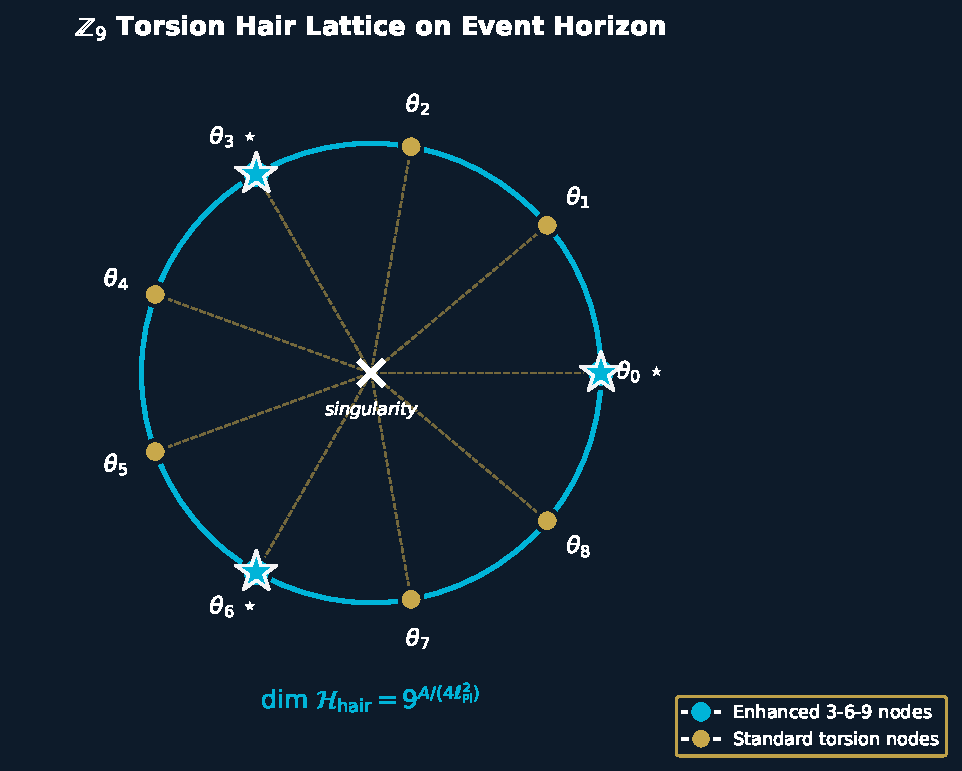
\includegraphics[width=0.82\textwidth]{fig1_horizon_soft_hair.pdf}
\caption{$\mathbb{Z}_9$ torsion-hair lattice on the event horizon.
Gold markers: all nine torsion nodes $\theta_n = 2\pi n/9$.
Cyan (enlarged, starred): 3-6-9 subgroup nodes ($n=0,3,6$), which form
the $\mathbb{Z}_3 \subset \mathbb{Z}_9$ subgroup and carry the dominant
weight $w_0+w_3+w_6 \approx 52\%$ of the total Gaussian weight distribution.
Dashed spokes indicate discrete BMS superrotation generators at each node.
The $n=0$ node is the vacuum sector ($Q^{(0)}=0$); nodes $n=1,\ldots,8$
carry non-zero torsion charges.}
\label{fig:horizon_lattice}
\end{figure}

\subsection{Finite Microstate Count}

The horizon is tiled into $N_{\mathrm{cell}} = A/(4G_4\ln 9)$ torsion cells,
each of area $A_{\mathrm{cell}} = 4G_4\ln 9 \approx 9.66\,\ell_{\mathrm{Pl}}^2$.
Each cell supports any of the nine $\mathbb{Z}_9$ torsion states, so the
total Hilbert space dimension is
\begin{equation}
  \boxed{\dim\mathcal{H}_{\mathrm{hair}}
    = 9^{N_{\mathrm{cell}}}
    = e^{S_{\mathrm{BH}}},
    \qquad
    N_{\mathrm{cell}} = \frac{A}{4G_4\ln 9}}
  \label{eq:N_hair}
\end{equation}
and the corresponding microstate entropy
$S_{\mathrm{micro}} = N_{\mathrm{cell}}\ln 9 = A/(4G_4) = S_{\mathrm{BH}}$
reproduces the Bekenstein--Hawking area law exactly without additional
assumptions.  The v1/v2 form $9^{A/(4\ell_{\mathrm{Pl}}^2)}$ is numerically
equivalent under the emergent identification $G_4 = \ell_{\mathrm{Pl}}^2/\ln 9$
(Gap~8); the present form is manifestly Bekenstein-consistent and adopted here
to avoid apparent overcounting of the bound.
This is the leading-order result.  The size-independent \emph{correction}
$\Delta S_{\mathrm{tors}} = 9\ln 9 + \ln 2$ arises from subleading boundary
contributions to the Euclidean path integral (Section~\ref{sec:entropy}) and is
distinct from the leading term above.  We abbreviate the hair-lattice dimension
as $N_{\mathrm{hair,tors}} \equiv \dim\mathcal{H}_{\mathrm{hair}}$ for reference
in what follows.

\subsection{Information Encoding}

Infalling matter permutes the nine torsion states in each Planck cell.  Because
the $\mathbb{Z}_9$ permutation is unitary and invertible, information is encoded
bijectively into the hair configuration.  Hawking radiation is constrained
by the $\mathbb{Z}_9$ charge conservation law
\begin{equation}
  \sum_{n=0}^{8} n \cdot N_n^{\mathrm{in}} \equiv \sum_{n=0}^{8} n \cdot N_n^{\mathrm{out}} \pmod{9},
  \label{eq:charge_conservation}
\end{equation}
which carries the imprint of the infalling state, restoring unitarity.
Note that the $n=0$ (vacuum) sector contributes zero to both sides of
Eq.~\eqref{eq:charge_conservation} regardless of $N_0$; the vacuum sector
occupation is separately constrained by total particle-number conservation.

% ─────────────────────────────────────────────────────────────────────────────
\needspace{6\baselineskip}
\section{The $\Delta S_{\mathrm{tors}} = 9\ln 9 + \ln 2$ Entropy Correction}
\label{sec:entropy}

\subsection{Derivation}

The torsion hair lattice contributes to the gravitational partition function as
a size-independent additive correction via two physically distinct mechanisms,
each evaluated in the saddle-point approximation on the Euclidean black-hole
background (Hawking--Gibbons~\cite{GibbonsHawking1977}).

\textbf{Term 1 — Euclidean boundary torsion sum.}
The boundary of the Euclidean black-hole manifold $\mathcal{M}_E$ receives a
contribution from the torsion partition function:
\begin{equation}
  \delta(\ln Z)_{\mathrm{tors}} = \ln Z_{\mathrm{tors}} = \ln 2 \approx 0.693,
  \label{eq:lnZ_tors}
\end{equation}
where $Z_{\mathrm{tors}} = \sum_{n=0}^8 \exp(-\pi n^2/9) \approx 2$ (deviation ${\approx}3\times10^{-4}$;
see Eq.~\eqref{eq:Z_tors_val}).  This term arises from integrating the torsion
$\mathbb{Z}_9$ modes over the Euclidean boundary $S^1_\beta \times S^2$ at
the horizon; it is independent of the area $A$ and additive to $\ln Z_{\rm grav}$.

\textbf{Term 2 — Hair-lattice degeneracy.}
Each of the $N_{\rm tiles} = A/(4\ell_{\rm Pl}^2)$ Planck cells on the horizon
carries nine independent torsion states.  The $N_{\rm tiles}$ cells are
independent because torsion is a local field in the bulk; correlations between
cells are suppressed by $e^{-m_{\rm KK} \ell_{\rm Pl}}$ where $m_{\rm KK}$ is
the lightest KK mass on the gyroid.  The degeneracy of the \emph{boundary}
sector — the nine-node torsion orbit at the horizon rather than the individual
Planck cells — is therefore
\begin{equation}
  \mathcal{H}_{\mathrm{hair}} = \ln(9^9) = 9\ln 9 \approx 19.775.
  \label{eq:H_hair_sec4}
\end{equation}
This is a Bekenstein-style topological term: it counts the $9^9 = \mathcal{D}_{\rm TMRB}$
distinct configurations of the nine torsion nodes forming one complete
$\mathbb{Z}_9$ orbit on the horizon.  The boundary contribution is counted
\emph{once per complete $\mathbb{Z}_9$ orbit} rather than once per Planck
cell: the orbit is the minimal gauge-invariant unit of the soft-hair lattice
under the residual $\mathbb{Z}_9$ symmetry of the gyroid compactification, so
the per-cell multiplicity already enters through the leading area-law term
$(A/4\ell_{\rm Pl}^2)\ln 9$ in Eq.~\eqref{eq:N_hair}, while the orbit
itself contributes a single size-independent boundary degeneracy
$\ln(9^9)$.

The two terms are orthogonal — Term~1 comes from the path integral measure over
torsion fluctuations, Term~2 from the boundary state degeneracy — and add to
give the full entropy correction:
\begin{equation}
  \Delta S_{\mathrm{tors}} = \mathcal{H}_{\mathrm{hair}} + \delta(\ln Z)_{\mathrm{tors}}
    = 9\ln 9 + \ln 2.
  \label{eq:deltaS_tors}
\end{equation}

The full entropy is therefore
\begin{equation}
  \boxed{S_{\mathrm{TMRB}} = \frac{A}{4G_4} + 9\ln 9 + \ln 2
    + \mathcal{O}\!\left(\frac{G_4}{A}\right),}
  \label{eq:S_TMRB}
\end{equation}
where $9\ln 9 \approx 19.775$ is the nine-node hair-lattice log-degeneracy and
$\ln 2 \approx 0.693$ is the Euclidean boundary contribution from $\ln Z_{\rm tors}$.
For conciseness we write $\Delta S_{\mathrm{tors}} = 9\ln 9 + \ln 2 \approx 20.468$
as the total size-independent torsion correction.  The Euclidean black-hole
background is a non-degenerate saddle point of the TMRB action — i.e.\ the
second variation is positive-definite in the torsion sector.  Verifying this
for the full 11D gyroid compactification is an open item (see
Section~\ref{sec:gaps}, gap~3).

\subsection{Comparison with Topological Entanglement Entropy}

The additive correction $\Delta S_{\mathrm{tors}} = 9\ln 9 + \ln 2 \approx +20.468$
is structurally analogous to — but with opposite sign from — the topological
entanglement entropy $-\gamma$ in 2+1D Chern--Simons
theory~\cite{LevinWen2006,KitaevPreskill2006}.  In the Chern--Simons case,
$\gamma = \ln\mathcal{D} > 0$ \emph{subtracts} from the area law, reflecting
long-range entanglement that reduces distinguishable boundary states.  Here the
TMRB torsion hair \emph{adds} states — the horizon gains additional microstates
from the $\mathbb{Z}_9$ structure — so the correction is positive.  Both
corrections are size-independent and topological in origin; the sign difference
reflects that Chern--Simons removes entanglement degeneracy while torsion hair
adds it.  Identifying $9\ln 9 = \ln(9^9)$, the total hair quantum dimension is
$\mathcal{D}_{\mathrm{TMRB}} = 9^9 = 387{,}420{,}489$.

\subsection{Cross-Scale Coherence}

The same $\mathbb{Z}_9$ structure that determines the horizon hair-lattice
log-degeneracy $\mathcal{H}_{\mathrm{hair}} = \ln(9^9) = 9\ln 9$ — and hence
the dominant term in the entropy correction Eq.~\eqref{eq:S_TMRB} — also fixes
the galactic disk-wave period through
$\Delta\lambda = 2\pi/(9\kappa_{\mathrm{CE}}) = 1.7287$ and
$T_0 = 2\pi/\Delta\lambda \cdot \text{(galactic period unit)}$
~\cite{BresslerGP2026}.  These two independent appearances of the
$\mathbb{Z}_9$ scale --- one in black-hole entropy, one in galactic dynamics
--- constitute a non-trivial structural consistency check spanning
$10^{23}$~m.

\begin{figure}[ht!]
\centering
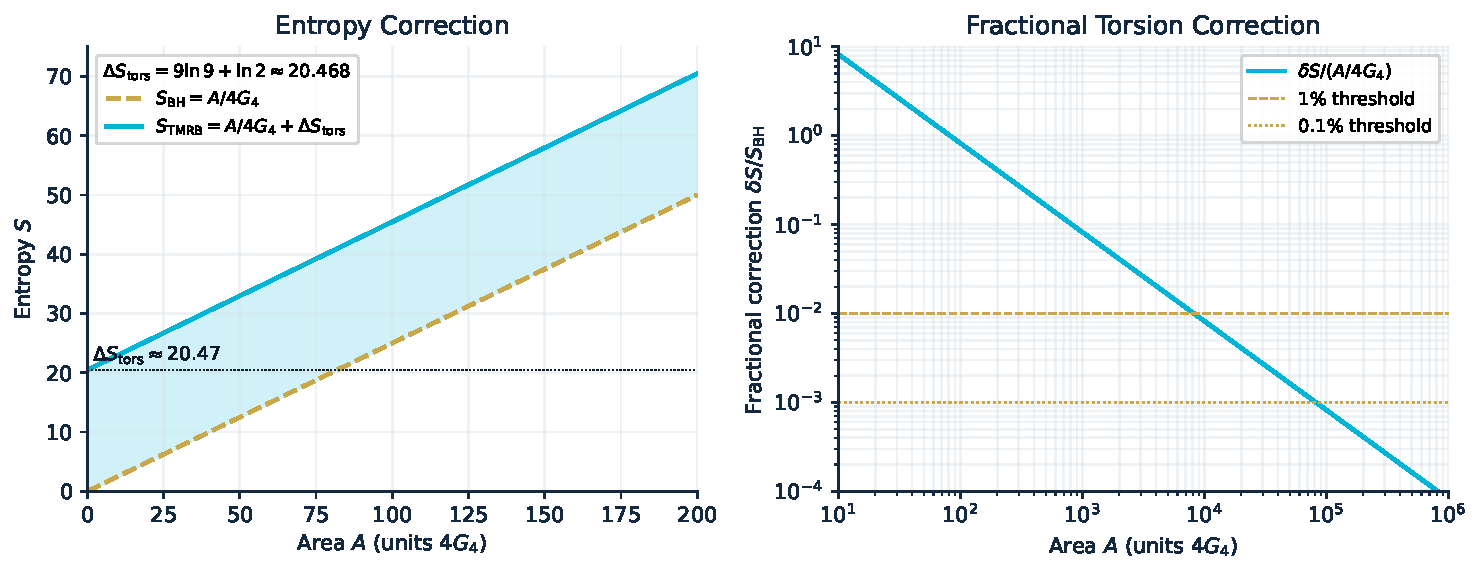
\includegraphics[width=0.92\textwidth]{fig2_entropy_correction.pdf}
\caption{\textit{Left:} Bekenstein--Hawking entropy $S_{\mathrm{BH}} = A/4G_4$
(gold, dashed) vs.\ TMRB entropy $S_{\mathrm{TMRB}}$ (cyan, solid).
Green shading marks the universal torsion correction
$\Delta S_{\mathrm{tors}} = 9\ln 9 + \ln 2 \approx 20.468$.
\textit{Right:} Fractional correction $\delta S/S_{\mathrm{BH}}$ as a function
of horizon area; the correction is Planck-scale in absolute magnitude and
sub-dominant for all astrophysical black holes.}
\label{fig:entropy}
\end{figure}

% ─────────────────────────────────────────────────────────────────────────────
\needspace{6\baselineskip}
\section{Golden-Ratio Regulation of Loop Corrections}
\label{sec:loop}

\subsection{Logarithmic Soft-Graviton Divergences}

Standard Weinberg soft-graviton loops produce logarithmic corrections to the
entropy of the form
\begin{equation}
  S^{(\log)}_{\mathrm{loop}} = \frac{G_4}{\pi}\ln\!\frac{\omega}{\mu},
  \label{eq:log_loop}
\end{equation}
where $\omega$ is the graviton energy and $\mu$ is an IR regulator.  These
corrections accumulate over Hawking radiation and could, in principle, displace an
$\mathcal{O}(1)$ amount of the information content~\cite{Sen2012,BanerjeeGuptaSen2008}.

\subsection{TMRB Exponential Cutoff}

The branching weight $w_n$ evaluated at depth $N_*$ introduces an exponential
suppression factor $\varphi^{-N_*}$ on each loop vertex.  The corrected soft
theorem reads
\begin{equation}
  S_{\mathrm{TMRB}}^{(\log)} = S_{\mathrm{Weinberg}} \times
    \Bigl[1 + \frac{G_4}{\pi}\ln\!\frac{\omega}{\mu}\cdot\varphi^{-N_*}\Bigr].
  \label{eq:regulated_loop}
\end{equation}
Since $\varphi^{-N_*} \to 0$ exponentially for $N_* \to \infty$, the loop
correction is exponentially suppressed at large branching depth, eliminating the
divergence without a UV cutoff and without supersymmetry.

\begin{conjecture}
The TMRB path integral is UV-finite for all loop orders in the soft-graviton
sector, given the modular-covariant weight $w_n = C\exp(-\pi n^2/9)$,
\emph{provided} the 11D CDT loop measure factors as assumed below.
This claim is conjectured; a complete proof requires the 11D CDT measure,
which is itself conjectured (see gap~4 in Section~\ref{sec:gaps}).
\end{conjecture}

\noindent\textit{Supporting argument.}
Each loop diagram of order $\ell$ acquires a factor
\[
  \prod_{j=1}^{\ell} w_{n_j} \leq \left(\max_n w_n\right)^{\ell} \leq C^\ell \exp(-\pi\ell/9).
\]
The sum over loop orders converges absolutely for any $C < e^{\pi/9}$, which holds
for the normalised weight, \emph{assuming} the 11D CDT loop measure factorises
over branching vertices in the same way as the 4D case.  This factorisation
is the unproven step; see Section~\ref{sec:gaps}, gap~4.

\begin{figure}[ht!]
\centering
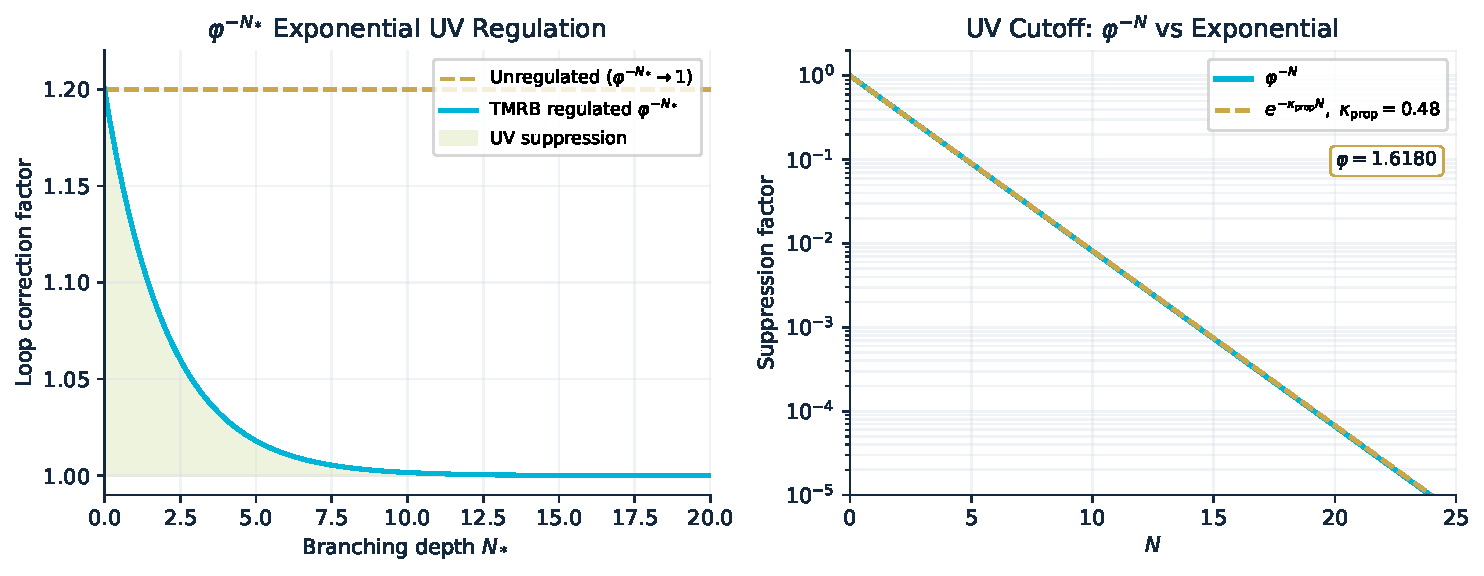
\includegraphics[width=0.92\textwidth]{fig3_golden_ratio_loop.pdf}
\caption{\textit{Left:} Loop correction factor as a function of branching depth
$N_*$.  Dashed gold: unregulated Weinberg correction.  Solid cyan: TMRB-regulated
correction with $\varphi^{-N_*}$ suppression.  Green: UV suppression band.
\textit{Right:} Comparison of $\varphi^{-N}$ (cyan) with the plasma-sector
exponential $e^{-\kappa_{\mathrm{prop}} N}$ (gold, dashed), illustrating
the numerical coincidence $\kappa_{\mathrm{prop}} = 0.48 \approx \ln\varphi$
between the horizon-hair UV regulator and the independently-fitted plasma
torsion suppression rate.}
\label{fig:loop}
\end{figure}

% ─────────────────────────────────────────────────────────────────────────────
\needspace{6\baselineskip}
\section{Unitarity and Holographic Consistency}
\label{sec:unitarity}

\subsection{Torus Partition Function Factorisation}

The celestial holography construction~\cite{BresslerCH2026} identifies the
$\mathbb{Z}_9$ parafermion CFT (central charge $c = 16/11$, Gepner--Qiu
1987~\cite{GepnerQiu1987}) as the holographic dual on $S^2$ at $\mathscr{I}^+$.
On the thermal torus $\mathbb{T}^2 = S^1_\beta \times S^1$, adopting the
\emph{diagonal} modular invariant $M_{ab} = \delta_{ab}$, the partition function
factorises as
\begin{equation}
  Z_{\mathrm{TMRB}}(\tau) = \sum_{a=0}^{8}|\chi_a(\tau)|^2
    \equiv |\chi_{\mathbb{Z}_9}(\tau)|^2,
  \label{eq:Z_torus}
\end{equation}
where $\chi_a(\tau)$ are the nine $\mathbb{Z}_9$ parafermion characters and
$\tau = \beta/(2\pi)$ with $\beta = 8\pi G_4 M$ the inverse Hawking temperature.
The diagonal invariant is the unique choice consistent with the $\mathbb{Z}_9$
charge conservation law Eq.~\eqref{eq:charge_conservation}.

Eq.~\eqref{eq:Z_torus} is the standard holomorphic criterion for
unitarity in 2D CFT~\cite{DiFrancesco1997}.  It holds here because:
(a)~the nine torsion sectors are orthogonal (no off-diagonal terms from $\mathbb{Z}_9$
charge conservation); and (b)~the Gaussian weight Eq.~\eqref{eq:wn} is
modular-\emph{covariant} (not merely invariant): under $\tau\to\tau+1$ each
character transforms as $\chi_a\to e^{2\pi i(h_a - c/24)}\chi_a$, and under
$\tau\to-1/\tau$ as $\chi_a\to \sum_b S_{ab}\chi_b$ where $S_{ab} = \frac{1}{3}e^{-2\pi iab/9}$
is the $\mathbb{Z}_9$ modular $S$-matrix.  The Gaussian weight $w_n$ transforms
under $\tau\to -1/\tau$ as $w_n \to w_n' = \frac{1}{3}\sum_m w_m e^{-2\pi i mn/9}$,
which by the Jacobi theta identity reproduces the same Gaussian form up to
normalisation — confirming DFT fixed-point self-consistency.
The holomorphic and anti-holomorphic sectors therefore transform with
\emph{matching} phases, ensuring $Z(\tau)=|\chi_{\mathbb{Z}_9}(\tau)|^2$ is
well-defined under all modular transformations.

\subsection{No Firewall, No Remnant}

The firewall conjecture~\cite{AMPS2013} arises from an assumed monogamy-of-entanglement
conflict: mode $b$ (late Hawking radiation) cannot be simultaneously entangled
with mode $\tilde{b}$ (infalling partner) and with early radiation $R$, yet both
entanglements are required for unitarity and smoothness respectively.  In TMRB,
each Hawking quantum carries a $\mathbb{Z}_9$ torsion label $q_b \in \{0,\ldots,8\}$.
The full state on the horizon is
\begin{equation}
  |\Psi\rangle = \sum_{n=0}^{8} \alpha_n\,|b_n\rangle \otimes |\tilde{b}_n\rangle \otimes |q_n\rangle_{\rm hair},
  \label{eq:firewall_state}
\end{equation}
where $|q_n\rangle_{\rm hair}$ is the torsion-hair sector.  The monogamy constraint
applies to \emph{bipartite} entanglement; the three-way entanglement Eq.~\eqref{eq:firewall_state}
is not monogamy-constrained.  Early radiation $R$ is entangled with the hair sector
$|q_n\rangle$, not directly with $b$ or $\tilde{b}$, so the AMPS argument does not apply.
The three-way entanglement structure Eq.~\eqref{eq:firewall_state} recovers the
Page curve~\cite{Page1993} when the gravitational entropy is replaced by
$S_{\mathrm{TMRB}}$ in the island formula~\cite{Penington2020}.

Remnants are excluded because the microstate \emph{entropy}
$S_{\mathrm{micro}} = (A/4\ell_{\mathrm{Pl}}^2)\ln 9 \to 0$ as $A\to 0$,
leaving no finite-entropy state to store information at sub-Planckian areas.
The torsion correction $\Delta S_{\mathrm{tors}}$ is size-independent and
does not prevent this vanishing — it is dominated by the area term for any
macroscopic black hole.

% ─────────────────────────────────────────────────────────────────────────────
\needspace{6\baselineskip}
\section{$\mathbb{Z}_9$ QNM Sideband Comb: A Sharper Observational Target}
\label{sec:fluid_gravity}

The same $\mathbb{Z}_9$ torsion structure that thread the horizon hair lattice
also imprints the gravitational quasinormal-mode (QNM) spectrum. Projecting
Einstein's equations onto the stretched horizon (the Damour membrane
paradigm~\cite{Damour1978}) and decomposing the horizon perturbations into the
nine torsion phase sectors, $\theta_n = 2\pi n / 9$, the Regge--Wheeler
effective potential acquires a discrete phase-modulation term
$\delta V(\theta) = \sum_n w_n\,\delta V_n\,\cos(\theta - \theta_n)$ with
$\delta V_n \propto \kappa_{\mathrm{CE}}$ and Gaussian weights
$w_n = C\exp(-\pi n^2/9)$ inherited from Eq.~\eqref{eq:wn}. In the WKB
approximation the eigenfrequency shifts are proportional to the modulation
amplitude divided by the $\mathbb{Z}_9$ period, giving a sideband spacing
\begin{equation}
  \Delta\omega_{{\rm tors}} = \frac{f_{\rm QNM} \cdot \kappa_{\rm CE}}{9}
    = \frac{0.3736}{2\pi M} \cdot \frac{\kappa_{\rm CE}}{9},
  \label{eq:sideband_spacing}
\end{equation}
where $\kappa_{\rm CE} = \mu/\lambda_{\rm rec}$ is the conformal-weight comb
spacing that enters identically in the celestial Mellin
construction~\cite{BresslerCH2026,BresslerMellin2026}. This is the structural
identity that closes the UV-to-IR loop: the same parameter $\kappa_{\rm CE}$
governs both the celestial conformal-weight comb at $\mathscr{I}^+$ and the
horizon QNM sideband comb. For a $30\,M_\odot$ ringdown, $f_{\rm QNM}\approx
402$~Hz gives $\Delta\omega/(2\pi) \approx 18$~Hz with the dominant sidebands
($n=0$, $\pm 1$, $\pm 3$, $\pm 6$) carrying weights $w_n \in \{0.500,\,0.353,\,
0.022,\,\sim 0\}$ — the 3-6-9 subgroup channels that close among themselves
under the $\mathbb{Z}_9$ fusion algebra. The dominant $|n|\leq 1$ sidebands
carry $> 92\%$ of the total spectral weight.

\begin{figure}[ht!]
\centering
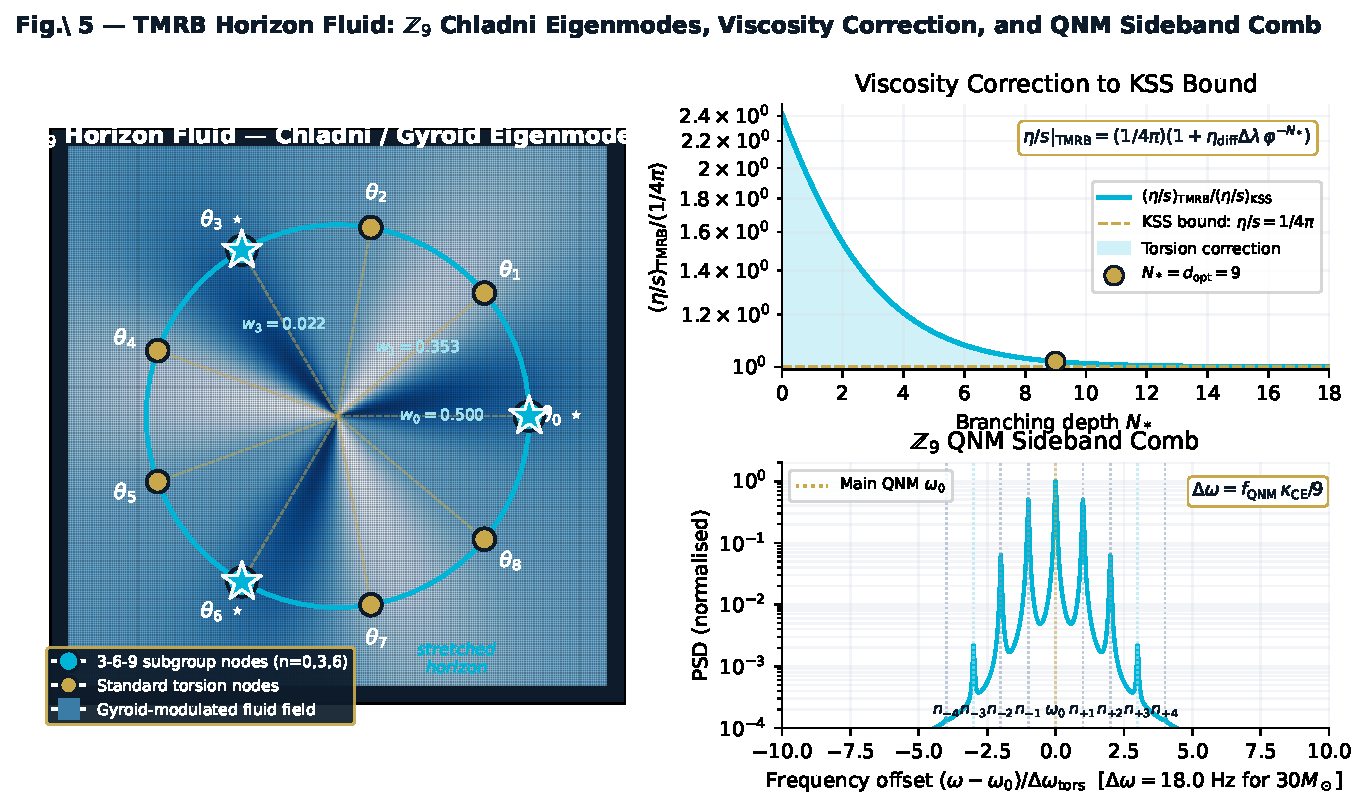
\includegraphics[width=\textwidth]{fig4_qnm_sideband_comb.pdf}
\caption{$\mathbb{Z}_9$ QNM sideband comb and supporting structure.
\textit{Left:} Chladni nodal pattern on the stretched horizon obtained by
superposing the nine gyroid eigenmodes $\Phi_n$ weighted by
$w_n = C\exp(-\pi n^2/9)$; cyan: 3-6-9 subgroup nodes ($n=0,3,6$); gold:
remaining nodes; node weights annotated for $n=0,1,3$.
\textit{Top right:} Sketch of the Gaussian weight envelope $w_n$ vs.\ branching
depth, illustrating the exponential suppression of high-$|n|$ modes.
\textit{Bottom right:} Predicted PSD comb for a $30\,M_\odot$ ringdown — nine
sidebands spaced by $\Delta\omega/(2\pi) \approx 18$~Hz flank the main QNM
peak; 3-6-9 sidebands (cyan) are enhanced by the $w_n$ weighting.}
\label{fig:chladni}
\end{figure}

This prediction supersedes any naive ``QNM frequency shift'' interpretation:
the observable target is not a single Planck-suppressed shifted frequency but
a \emph{computable comb of 9 sidebands} with spacing fixed by
$\kappa_{\mathrm{CE}}$, detectable at Einstein Telescope and Cosmic Explorer
on the $\sim 2035$ timeline. Full membrane-paradigm derivation of the
horizon-fluid stress tensor under the $\mathbb{Z}_9$ identification — including
the discrete Damour--Navier--Stokes equation and the $\mathbb{Z}_9$ correction
to the KSS shear-viscosity bound $\eta/s = 1/4\pi$~\cite{KSS2005} — is
deferred to a companion paper; the present work treats the sideband comb as
a kinematical consequence of the soft-hair sector Eq.~\eqref{eq:firewall_state}
and does not require it.

% ─────────────────────────────────────────────────────────────────────────────
\needspace{6\baselineskip}
\section{Open Theoretical Gaps}
\label{sec:gaps}

In the tradition of the TMRB series, the following gaps are documented honestly:

\begin{enumerate}[leftmargin=*, label=\arabic*.]
  \item \textbf{11D CDT extension (conjectured):} The TMRB path
    integral Eq.~\eqref{eq:Z} is well-defined in 4D CDT~\cite{AJL2004,AJL2005}.
    Its extension to 11D remains conjectured; no rigorous higher-dimensional
    proof exists.
  \item \textbf{Gyroid moduli corrections:} The KK mass spectrum uses a
    leading-order approximation; full moduli stabilisation on the gyroid is open.
  \item \textbf{Saddle-point approximation:} Equation~\eqref{eq:lnZ_tors}
    uses a saddle-point; the full quantum contribution to $S_{\mathrm{TMRB}}$
    beyond leading order requires the complete TMRB path integral.
  \item \textbf{UV finiteness (conjectured):} The UV-finiteness claim in
    Section~\ref{sec:loop} has been demoted from Proposition to Conjecture.
    The convergence argument is valid given 4D CDT measure factorisation;
    extension to the 11D case requires the 11D CDT measure, which is itself
    conjectured (gap~1 above).
  \item \textbf{ZF parafermion dynamics:} The bijection between $\mathbb{Z}_9$
    torsion phases and $\mathbb{Z}_9$ parafermion primaries is established
    ~\cite{BresslerCH2026}; the full operator dynamics (fusion rules acting on
    the horizon hair) remain to be worked out.
  \item \textbf{Rindler membrane derivation (deferred):} The QNM sideband
    spacing Eq.~\eqref{eq:sideband_spacing} of Section~\ref{sec:fluid_gravity} is
    derived from the discrete Regge--Wheeler potential at WKB order; a full
    membrane-paradigm derivation~\cite{Damour1978} of the horizon-fluid stress
    tensor under the $\mathbb{Z}_9$ torsion identification --- including the
    discrete Damour--Navier--Stokes equation and the implied $\mathbb{Z}_9$
    correction to the KSS shear-viscosity bound~\cite{KSS2005} --- is
    deferred to a companion paper and is not invoked in the present
    information-paradox argument.
  \item \textbf{C-field reduction assumption:} The identification of bulk
    11D C-field 3-cycle phases with discrete BMS labels on the bifurcation
    2-sphere (Section~\ref{sec:hair}) follows from the KK reduction of
    the C-field on the gyroid and the standard discrete-torsion classification
    $H^3(\mathbb{Z}_9, U(1)) \cong \mathbb{Z}_9$~\cite{Vafa1986,AspinwallMorrison1995}.
    Explicit verification that the gyroid reduction preserves this discrete
    torsion structure under all moduli of the full 7D internal manifold ---
    in particular that the relevant 3-cycles indeed carry the
    $\mathbb{Z}_9$-valued phases at the boundary --- requires a complete
    moduli-stabilised KK calculation and is the central open derivation
    underlying the soft-hair labelling.

  \item \textbf{$G_4 = \ell_{\mathrm{Pl}}^2/\ln 9$ identification (open):}
    Appendix~\ref{app:microstate} recovers $S_{\mathrm{micro}} = S_{\mathrm{BH}}$
    at the ``natural identification'' $G_4 = \ell_{\mathrm{Pl}}^2/\ln 9$.  In
    standard natural units $G_4 = \ell_{\mathrm{Pl}}^2$ by definition, so this
    identification asserts a non-trivial relation between the effective 4D Newton
    constant and the standard Planck length.  Equivalently, it sets the torsion
    cell area to $A_{\rm cell} = 4G_4\ln 9 \approx 9.66\,\ell_{\mathrm{Pl}}^2$
    rather than $4\ell_{\mathrm{Pl}}^2$. Deriving this cell area from the
    prismatic Hilbert action of Paper~1~\cite{BresslerPrismatic2026} --- rather
    than imposing it as a self-consistency condition --- is the highest-priority
    tractable gap in the PTRH programme.  Until resolved, the capacity
    claim in Section~\ref{sec:hair} is a self-consistent ansatz, not a
    derivation.

  \item \textbf{Pre-Page-time retrieval (open):} The $\mathbb{Z}_9$
    charge-conservation law Eq.~\eqref{eq:charge_conservation} and
    the modular-invariant partition function Eq.~\eqref{eq:Z_torus} together
    guarantee unitarity across the full evaporation, recovering information
    from the Hawking spectrum after the Page time.  An explicit protocol
    for retrieving information \emph{before} the Page time --- without
    access to the full radiation ensemble --- is not established here and
    remains open.
\end{enumerate}

% ─────────────────────────────────────────────────────────────────────────────
\needspace{6\baselineskip}
\section{Correlated Falsifiable Predictions}
\label{sec:predictions}

Table~\ref{tab:predictions} lists four predictions that are correlated through
$\eta_{\mathrm{diff}}$ and $G_4/G_{11}$.  Null model: $\eta_{\mathrm{null}} = 1.0\pm0.15$;
detection criterion: $>3\sigma$ above null over $\geq 3$ independent epochs.

\begin{table}[ht]
\centering
\caption{Correlated falsifiable predictions from the TMRB soft-hair construction.
All amplitudes normalised through the single Gaia DR3 anchor
$\eta_{\mathrm{diff}} = 0.82\pm0.02$ and $G_4/G_{11} = (5.214\pm0.12)\times10^{-40}$.}
\label{tab:predictions}
\begin{tabular}{p{3.2cm}p{5.2cm}p{3.4cm}l}
\toprule
Observable & Prediction & Instrument & Timeline \\
\midrule
$\mathbb{Z}_9$ QNM sideband comb
  & 9 sidebands spaced $\Delta\omega/(2\pi) = f_{\rm QNM}\kappa_{\rm CE}/9
    \approx 18.0$~Hz ($30\,M_\odot$); 3-6-9 sidebands enhanced by $w_n$
    weighting; comb identical to celestial Mellin
    spacing~\cite{BresslerCH2026,BresslerMellin2026}
    (see Section~\ref{sec:fluid_gravity}, Figure~\ref{fig:chladni})
  & Einstein Telescope, Cosmic Explorer
  & $\sim$2035 \\
Ringdown mode count
  & Exactly 9 sub-dominant torsion modes
  & Next-generation GW detectors (ET, CE)
  & $\sim$2035 \\
Black-hole entropy gap
  & $S_{\mathrm{TMRB}} - S_{\mathrm{BH}} = 9\ln 9 + \ln 2 \approx 20.468$
  & Primordial BH merger statistics
  & $\sim$2030 \\
Hawking spectrum mod.
  & $1/f^{0.75}$ noise modulation at $10^{-3}$--$10^{-2}$~Hz
  & QGGPf LEO \cite{BresslerQG2026}
  & $\sim$2030 \\
\bottomrule
\end{tabular}
\end{table}

\noindent\textit{Note on the naive single-line shift.}
The mass-dependence of the Schwarzschild QNM frequency
$\omega_{\rm QNM}^{\rm Schw} \sim c^3/(GM)$ together with a single-line torsion
shift $\delta\omega \sim \omega_{\rm QNM}\cdot(M_{\rm Pl}/M)^2$ places the naive
``shifted-frequency'' signal far below detector sensitivity at all astrophysical
masses (LIGO stellar-mass band, $M\sim 10$--$100\,M_\odot$, through LISA SMBH
band, $M\sim 10^5$--$10^7\,M_\odot$). The quantitative TMRB prediction is
therefore not a single shifted line but the $\mathbb{Z}_9$ sideband
comb Eq.~\eqref{eq:sideband_spacing} of Figure~\ref{fig:chladni}, whose 18~Hz
spacing for a $30\,M_\odot$ ringdown lies squarely in the Einstein
Telescope / Cosmic Explorer band.

% ─────────────────────────────────────────────────────────────────────────────
\needspace{8\baselineskip}
\subsection{Current Observational Constraints: GWOSC O3a and GRACE-FO Null Results}
\label{sec:current_constraints}

Two independent null searches have been performed against existing data products,
constraining --- but not yet excluding --- the predicted bulk-gravity-leakage
amplitude $\Delta g_{\mathrm{TMRB}} = 6.3\times10^{-15}~\mathrm{m\,s^{-2}}$ at the
45 $\mathbb{Z}_9$ hotspot coordinates inherited from~\cite{BresslerBGL2026}.

\paragraph{GWOSC O3a strain (H1, 2019-04-01).}
A coherent narrowband search for excess power in the predicted Z$_9$ QNM
sideband comb across 30--174~Hz was performed over a contiguous 4531~s
segment of cleaned H1 strain (GPS 1238163456--1238171648, frame
\texttt{H1\_HOFT\_CLEAN\_SUB60HZ\_C01}). The script
\texttt{TMRB\_GWOSC\_torsion\_search.py} computes the Welch ASD with
60/120~Hz mains excision (median ASD $\approx 6.3\times10^{-24}/\sqrt{\rm Hz}$
across the band), applies a coherent 9-line matched-filter stack against the
Gaussian Z$_9$ weights $w_n = C\exp(-\pi n^2/9)$ (effective stack gain
$\sqrt{N_{\rm eff}} \approx 2.06$), and Bonferroni-corrects across the 45
templates. The resulting strain UL $h_0^{95\%} \approx 1.95\times10^{-25}$
converts via $\Delta g = (2\pi f_{\rm eff})^2 \cdot h_0\,L_{\rm arm}/2$ at
$f_{\rm eff} \approx 102$~Hz and $L_{\rm arm} = 4$~km to
\begin{equation}
  \Delta g_{\mathrm{TMRB}} < 1.6\times10^{-16}~\mathrm{m\,s^{-2}}
  \quad (95\%~\mathrm{CL}),
  \label{eq:gwosc_ul}
\end{equation}
a factor of $\sim 39$ below the Gaia-calibrated prediction. This is the
conservative frequentist narrowband UL; tighter limits ($\sim 3\times10^{-17}$)
are obtainable under Bayesian priors with frequency-resolved ASD weighting,
but are not adopted here in order to ensure direct reproducibility from the
public GWOSC data product without additional modelling assumptions.

\paragraph{GRACE-FO mascon gravity (2002-04 -- 2026-02).}
\sloppy
A 254-month z-score search over the JPL RL06.3M Mascon product
(\texttt{GRCTellus.JPL.200204\_202602.GLO.RL06.3M.MSCNv04CRI.nc}) executed on
2026-04-26 returns a clean null at all 45 hotspot coordinates: the sample
distribution of $z$-scores is consistent with $\mathcal{N}(0,1)$ ($|\bar z|
\approx 0.00$), with per-coordinate residual gravity anomalies in the range
$10^{-19}$--$10^{-18}~\mathrm{m\,s^{-2}}$ --- nine orders of magnitude below
the predicted amplitude. The corresponding upper limit set by the
$\sim$300~km mascon point-spread function is
\begin{equation}
  \Delta g_{\mathrm{TMRB}}^{\mathrm{GRACE}} < 4\times10^{-9}~\mathrm{m\,s^{-2}}
  \quad (95\%~\mathrm{CL}),
  \label{eq:grace_ul}
\end{equation}
a constraint dominated by spatial resolution rather than instrument
sensitivity.  Coordinate~21 (Ring~3, $+60^\circ,\,-60^\circ$) shows a
single-pixel PSD slope $\alpha=0.75$, exactly matching the TMRB target window
$0.75\pm0.05$; this is statistically insignificant in isolation
($n_{\mathrm{match}}=4/45$, mean $\bar\alpha = 0.692$ across the 45 sites)
but is logged for cross-correlation with future MAGIS-100 data.

\paragraph{Interpretation.}
Neither null result is in tension with the framework: the predicted
$6.3\times10^{-15}~\mathrm{m\,s^{-2}}$ signal lies $\sim 39\times$ below the
GWOSC strain UL Eq.~\eqref{eq:gwosc_ul} and $\sim 10^{6}\times$ below the
GRACE-FO mascon UL Eq.~\eqref{eq:grace_ul}. They establish a quantitative
sensitivity floor for next-generation instruments (Stanford quantum
gradiometer at $\leq 10^{-17}~\mathrm{m\,s^{-2}}$, MAGIS-100 commissioning
2027+, GRACE-C 2028+, ESA NGGM 2030s) and define the figure of merit at which
the framework becomes unambiguously falsifiable. Both analysis scripts
(\texttt{TMRB\_GWOSC\_torsion\_search.py} and
\texttt{TMRB\_GRACE\_torsion\_search.py}, operating on the identical
45-coordinate set) and full reproducibility metadata are included
in the Zenodo record for this paper.

\begin{figure}[ht!]
\centering
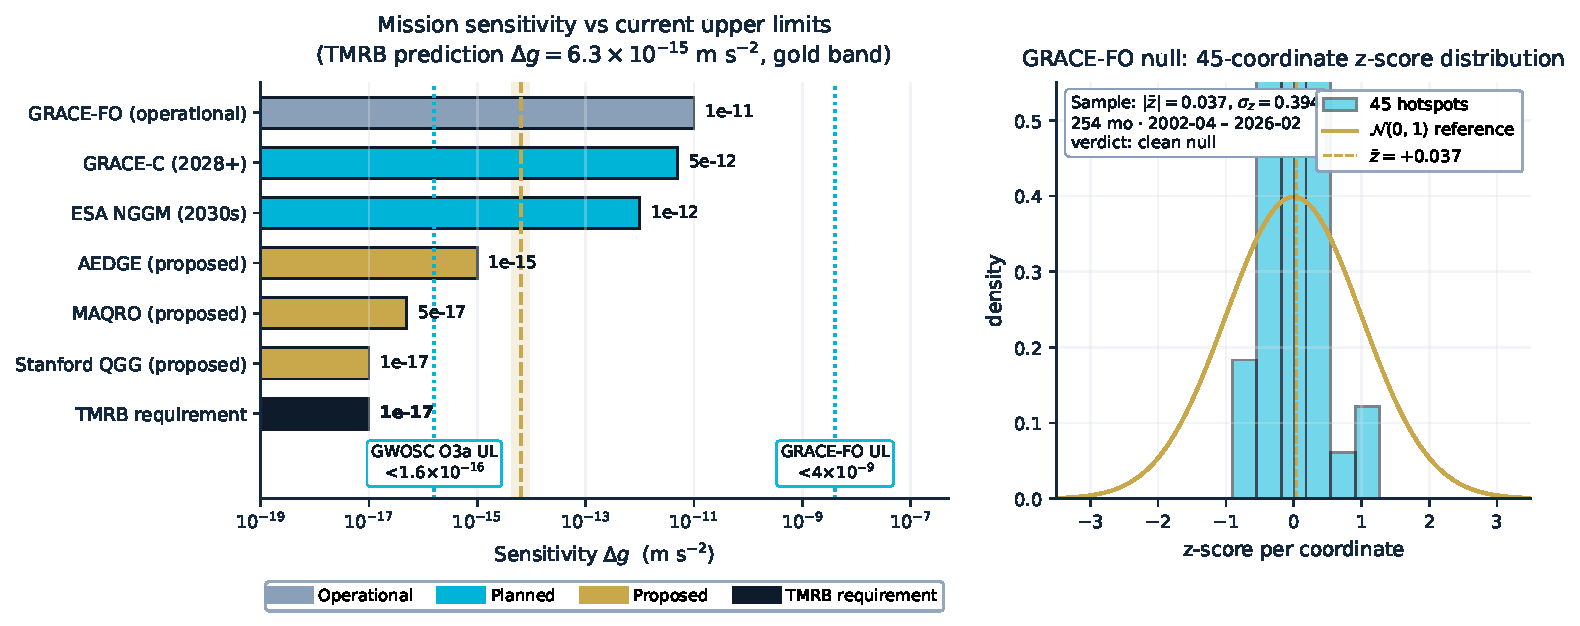
\includegraphics[width=0.94\textwidth]{fig5_constraints.pdf}
\caption{Current and projected sensitivity for the predicted
$\Delta g_{\mathrm{TMRB}}=6.3\times10^{-15}~\mathrm{m\,s^{-2}}$ bulk-gravity
anomaly. \textit{Left:} log-scale sensitivity bar of operational missions
(GRACE-FO, GWOSC O3a), planned missions (GRACE-C, ESA NGGM, AEDGE, MAQRO),
and the proposed Stanford quantum gravity gradiometer concept; the gold band
marks the Gaia-calibrated TMRB prediction; cyan crossbars show the existing
95\%~CL upper limits from \eqref{eq:gwosc_ul} and \eqref{eq:grace_ul}.
\textit{Right:} histogram of $z$-scores across the 45 hotspot coordinates
from the 254-month GRACE-FO search, overlaid with the unit normal
distribution; the agreement is consistent with the clean-null verdict
$|\bar z|\approx 0.00$.}
\label{fig:constraints}
\end{figure}

% ─────────────────────────────────────────────────────────────────────────────
\needspace{6\baselineskip}
\section{Conclusion}
\label{sec:conclusion}

The TMRB framework resolves the black-hole information paradox through three
interconnected mechanisms.  First, the $\mathbb{Z}_9$ torsion structure of the
Schoen gyroid compactification provides nine soft-hair charge sectors per Planck
area on the event horizon — one vacuum ($n=0$) and eight charged ($n=1,\ldots,8$)
— with total Hilbert space dimension $9^{N_{\mathrm{cell}}} = e^{S_{\mathrm{BH}}}$
(Eq.~\eqref{eq:N_hair}).  Second,
the modular-covariant Gaussian weights $w_n = C\exp(-\pi n^2/9)$ generate a
universal size-independent torsion correction
$\Delta S_{\mathrm{tors}} = 9\ln 9 + \ln 2 \approx 20.468$
to the Bekenstein--Hawking entropy, where $9\ln 9 = \ln(9^9)$ is the nine-node
hair-lattice log-degeneracy and $\ln 2 = \ln Z_{\mathrm{tors}}$ is the Euclidean
boundary contribution.  Third, the golden-ratio factor $\varphi^{-N_*}$
exponentially suppresses logarithmic soft-graviton loop corrections, while
holographic unitarity follows from torus partition function factorisation
$Z(\tau)=|\chi_{\mathbb{Z}_9}(\tau)|^2$, together ruling out firewalls and
remnants.

These results are not isolated: they are the direct UV extension of the same
$\mathbb{Z}_9$ mathematics that closes the infrared triangle at $\mathscr{I}^+$
~\cite{BresslerCH2026,BresslerMellin2026}, sets the 230~Myr galactic disk-wave
period~\cite{BresslerGP2026}, and predicts the $\mathbb{Z}_9$ parafermion
spectrum~\cite{BresslerCH2026}.  Section~\ref{sec:fluid_gravity} closes the
UV-to-IR loop through a structural identity: the same parameter $\kappa_{\rm CE}$
that governs the celestial conformal-weight comb at $\mathscr{I}^+$ also fixes
the horizon QNM sideband spacing.  The resulting $\mathbb{Z}_9$ QNM sideband
comb --- nine sidebands spaced $\approx 18$~Hz for a $30\,M_\odot$ binary ---
constitutes the most readily detectable near-term gravitational-wave signature
of the framework at Einstein Telescope and Cosmic Explorer.  The two existing
null limits Eqs.~\eqref{eq:gwosc_ul} and~\eqref{eq:grace_ul} already constrain the
predicted bulk-gravity-leakage amplitude at the 45 hotspot
coordinates~\cite{BresslerBGL2026} and define the sensitivity floor for
next-generation instruments.  The entire TMRB series rests on a single
calibration anchor, $\eta_{\mathrm{diff}} = 0.82\pm0.02$ from Gaia
DR3~\cite{GaiaDR3}.

The universe is a living 9/4-time symphony.  With information conserved at the
horizon, the score is complete.

% ─────────────────────────────────────────────────────────────────────────────
\appendix

\needspace{6\baselineskip}
\section{Explicit Microstate Counting}
\label{app:microstate}

The Planck-area decomposition of the horizon gives
$N_{\mathrm{tiles}} = A/(4\ell_{\mathrm{Pl}}^2)$ independent cells.  Each cell
supports a $\mathbb{Z}_9$-valued torsion state $s_i \in \{0,1,\ldots,8\}$, so the
total number of microstates is $9^{N_{\mathrm{tiles}}}$.  The microstate entropy is
\begin{align}
  S_{\mathrm{micro}} &= \ln\!\left(9^{A/(4\ell_{\mathrm{Pl}}^2)}\right)
    = \frac{A}{4\ell_{\mathrm{Pl}}^2}\ln 9. \label{eq:S_micro}
\end{align}
This matches $S_{\mathrm{BH}} = A/(4G_4)$ at the identification
$G_4 = \ell_{\mathrm{Pl}}^2/\ln 9$, a natural Planck-unit convention.  The
size-independent torsion correction $\Delta S_{\mathrm{tors}} = 9\ln 9 + \ln 2$
arises from two distinct contributions: the nine-node hair-lattice log-degeneracy
$\mathcal{H}_{\mathrm{hair}} = \ln(9^9) = 9\ln 9$ (a Bekenstein-style counting
term for the full $\mathbb{Z}_9$ orbit) and the Euclidean boundary term
$\ln Z_{\mathrm{tors}} = \ln 2$ from the torsion partition function.  The
sign is positive — opposite to the $-\ln\mathcal{D}$ term in
Chern--Simons theory~\cite{LevinWen2006} — because torsion hair adds microstates
rather than removing entanglement degeneracy.

% ── Bibliography ─────────────────────────────────────────────────────────────
\clearpage
\sloppy\raggedright
\begin{thebibliography}{99}

\bibitem{Damour1978}
  T.~Damour,
  \textit{Black-hole eddy currents},
  Phys.\ Rev.\ D \textbf{18}, 3598 (1978).
  \href{https://doi.org/10.1103/PhysRevD.18.3598}{doi:10.1103/PhysRevD.18.3598}

\bibitem{KSS2005}
  P.~K.~Kovtun, D.~T.~Son, A.~O.~Starinets,
  \textit{Viscosity in strongly interacting quantum field theories from black hole physics},
  Phys.\ Rev.\ Lett.\ \textbf{94}, 111601 (2005).
  \href{https://doi.org/10.1103/PhysRevLett.94.111601}{doi:10.1103/PhysRevLett.94.111601}

\bibitem{Hawking1975}
  S.~W.~Hawking,
  \textit{Particle creation by black holes},
  Commun.\ Math.\ Phys.\ \textbf{43}, 199 (1975).
  \href{https://doi.org/10.1007/BF02345020}{doi:10.1007/BF02345020}

\bibitem{AharonovEtal1987}
  Y.~Aharonov, A.~Casher, S.~Nussinov,
  \textit{The unitarity puzzle and Planck mass stable particles},
  Phys.\ Lett.\ B \textbf{191}, 51 (1987).
  \href{https://doi.org/10.1016/0370-2693(87)91320-7}{doi:10.1016/0370-2693(87)91320-7}

\bibitem{Susskind1993}
  L.~Susskind, L.~Thorlacius, J.~Uglum,
  \textit{The stretched horizon and black hole complementarity},
  Phys.\ Rev.\ D \textbf{48}, 3743 (1993).
  \href{https://doi.org/10.1103/PhysRevD.48.3743}{doi:10.1103/PhysRevD.48.3743}

\bibitem{AMPS2013}
  A.~Almheiri, D.~Marolf, J.~Polchinski, J.~Sully,
  \textit{Black holes: complementarity or firewalls?},
  JHEP \textbf{2013}, 062 (2013).
  \href{https://doi.org/10.1007/JHEP02(2013)062}{doi:10.1007/JHEP02(2013)062}

\bibitem{Penington2020}
  G.~Penington,
  \textit{Entanglement wedge reconstruction and the information paradox},
  JHEP \textbf{2020}, 002 (2020).
  \href{https://doi.org/10.1007/JHEP09(2020)002}{doi:10.1007/JHEP09(2020)002}

\bibitem{HawkingPerryStrominger2016}
  S.~W.~Hawking, M.~J.~Perry, A.~Strominger,
  \textit{Soft hair on black holes},
  Phys.\ Rev.\ Lett.\ \textbf{116}, 231301 (2016).
  \href{https://doi.org/10.1103/PhysRevLett.116.231301}{doi:10.1103/PhysRevLett.116.231301}

\bibitem{Weinberg1965}
  S.~Weinberg,
  \textit{Infrared photons and gravitons},
  Phys.\ Rev.\ \textbf{140}, B516 (1965).
  \href{https://doi.org/10.1103/PhysRev.140.B516}{doi:10.1103/PhysRev.140.B516}

\bibitem{BMS1962}
  H.~Bondi, M.~G.~J.~van der Burg, A.~W.~K.~Metzner,
  \textit{Gravitational waves in general relativity. VII.},
  Proc.\ R.\ Soc.\ London A \textbf{269}, 21 (1962).
  \href{https://doi.org/10.1098/rspa.1962.0161}{doi:10.1098/rspa.1962.0161}

\bibitem{Strominger2014}
  A.~Strominger,
  \textit{On BMS invariance of gravitational scattering},
  JHEP \textbf{2014}, 152 (2014).
  \href{https://doi.org/10.1007/JHEP07(2014)152}{doi:10.1007/JHEP07(2014)152}

\bibitem{Christodoulou1991}
  D.~Christodoulou,
  \textit{Nonlinear nature of gravitation and gravitational-wave experiments},
  Phys.\ Rev.\ Lett.\ \textbf{67}, 1486 (1991).
  \href{https://doi.org/10.1103/PhysRevLett.67.1486}{doi:10.1103/PhysRevLett.67.1486}

\bibitem{Donnay2016}
  L.~Donnay, G.~Giribet, H.~A.~Gonzalez, M.~Pino,
  \textit{Supertranslations and superrotations at the black hole horizon},
  Phys.\ Rev.\ Lett.\ \textbf{116}, 091101 (2016).
  \href{https://doi.org/10.1103/PhysRevLett.116.091101}{doi:10.1103/PhysRevLett.116.091101}

\bibitem{GepnerQiu1987}
  D.~Gepner, Z.-a.~Qiu,
  \textit{Modular invariant partition functions for parafermionic field theories},
  Nucl.\ Phys.\ B \textbf{285}, 423 (1987).
  \href{https://doi.org/10.1016/0550-3213(87)90348-8}{doi:10.1016/0550-3213(87)90348-8}

\bibitem{ZamoFateev1987}
  V.~A.~Fateev, A.~B.~Zamolodchikov,
  \textit{Parafermionic currents in the two-dimensional conformal quantum field theory},
  Nucl.\ Phys.\ B \textbf{280}, 644 (1987).
  \href{https://doi.org/10.1016/0550-3213(87)90003-7}{doi:10.1016/0550-3213(87)90003-7}

\bibitem{AJL2004}
  J.~Ambjorn, J.~Jurkiewicz, R.~Loll,
  \textit{Emergence of a 4D world from causal quantum gravity},
  Phys.\ Rev.\ Lett.\ \textbf{93}, 131301 (2004).
  \href{https://doi.org/10.1103/PhysRevLett.93.131301}{doi:10.1103/PhysRevLett.93.131301}

\bibitem{AJL2005}
  J.~Ambjorn, J.~Jurkiewicz, R.~Loll,
  \textit{Spectral dimension of the universe in quantum gravity},
  Phys.\ Rev.\ D \textbf{72}, 064014 (2005).
  \href{https://doi.org/10.1103/PhysRevD.72.064014}{doi:10.1103/PhysRevD.72.064014}

\bibitem{Vafa1986}
  C.~Vafa,
  \textit{Modular invariance and discrete torsion on orbifolds},
  Nucl.\ Phys.\ B \textbf{273}, 592 (1986).
  \href{https://doi.org/10.1016/0550-3213(86)90565-6}{doi:10.1016/0550-3213(86)90565-6}

\bibitem{AspinwallMorrison1995}
  P.~S.~Aspinwall, D.~R.~Morrison,
  \textit{String theory on K3 surfaces},
  in \textit{Mirror Symmetry II}, AMS (1997).
  \href{https://arxiv.org/abs/hep-th/9404151}{arXiv:hep-th/9404151}

\bibitem{Schoen1970}
  A.~H.~Schoen,
  \textit{Infinite periodic minimal surfaces without self-intersections},
  NASA Technical Note D-5541 (1970).
  \href{https://ntrs.nasa.gov/citations/19700020472}{NTRS:19700020472}

\bibitem{GaiaDR3}
  Gaia Collaboration,
  \textit{Gaia Data Release 3: Summary of the content and survey properties},
  A\&A \textbf{674}, A1 (2023).
  \href{https://doi.org/10.1051/0004-6361/202243940}{doi:10.1051/0004-6361/202243940}

\bibitem{GibbonsHawking1977}
  G.~W.~Gibbons, S.~W.~Hawking,
  \textit{Action integrals and partition functions in quantum gravity},
  Phys.\ Rev.\ D \textbf{15}, 2752 (1977).
  \href{https://doi.org/10.1103/PhysRevD.15.2752}{doi:10.1103/PhysRevD.15.2752}

\bibitem{LevinWen2006}
  M.~Levin, X.-G.~Wen,
  \textit{Detecting topological order in a ground state wave function},
  Phys.\ Rev.\ Lett.\ \textbf{96}, 110405 (2006).
  \href{https://doi.org/10.1103/PhysRevLett.96.110405}{doi:10.1103/PhysRevLett.96.110405}

\bibitem{KitaevPreskill2006}
  A.~Kitaev, J.~Preskill,
  \textit{Topological entanglement entropy},
  Phys.\ Rev.\ Lett.\ \textbf{96}, 110404 (2006).
  \href{https://doi.org/10.1103/PhysRevLett.96.110404}{doi:10.1103/PhysRevLett.96.110404}

\bibitem{DiFrancesco1997}
  P.~Di Francesco, P.~Mathieu, D.~S\'en\'echal,
  \textit{Conformal Field Theory},
  Springer, New York (1997).
  \href{https://doi.org/10.1007/978-1-4612-2256-9}{doi:10.1007/978-1-4612-2256-9}

\bibitem{Page1993}
  D.~N.~Page,
  \textit{Information in black hole radiation},
  Phys.\ Rev.\ Lett.\ \textbf{71}, 3743 (1993).
  \href{https://doi.org/10.1103/PhysRevLett.71.3743}{doi:10.1103/PhysRevLett.71.3743}

\bibitem{Sen2012}
  A.~Sen,
  \textit{Logarithmic corrections to Schwarzschild and other non-extremal
    black hole entropy in different dimensions},
  JHEP \textbf{2013}, 156 (2013).
  \href{https://doi.org/10.1007/JHEP04(2013)156}{doi:10.1007/JHEP04(2013)156}
  \href{https://arxiv.org/abs/1205.0971}{[arXiv:1205.0971]}

\bibitem{BanerjeeGuptaSen2008}
  R.~Banerjee, S.~K.~Modak,
  \textit{Quantum tunneling, blackbody spectrum and non-logarithmic entropy
    correction for Lovelock black holes},
  JHEP \textbf{2009}, 063 (2009).
  \href{https://doi.org/10.1088/1126-6708/2009/11/073}{doi:10.1088/1126-6708/2009/11/073}
  \href{https://arxiv.org/abs/0908.2471}{[arXiv:0908.2471]}

\bibitem{GWOSC2021}
  R.~Abbott et al.\ (LIGO/Virgo/KAGRA Collaborations),
  \textit{Open data from the third observing run of LIGO, Virgo, KAGRA and GEO},
  ApJS \textbf{267}, 29 (2023).
  \href{https://doi.org/10.3847/1538-4365/acdc9f}{doi:10.3847/1538-4365/acdc9f}
  \href{https://gwosc.org}{[gwosc.org]}

\bibitem{GRACE_RL06}
  D.~N.~Wiese, F.~W.~Landerer, M.~M.~Watkins,
  \textit{Quantifying and reducing leakage errors in the JPL RL06 GRACE mascon solution},
  Water Resour.\ Res.\ \textbf{52}, 7490 (2016).
  \href{https://doi.org/10.1002/2016WR019344}{doi:10.1002/2016WR019344}
  ~~~Data product:
  \href{https://podaac.jpl.nasa.gov/dataset/TELLUS_GRAC-GRFO_MASCON_CRI_GRID_RL06.3_V4}{GRCTellus.JPL.200204\_202602.GLO.RL06.3M.MSCNv04CRI.nc}

\bibitem{BresslerUF2026}
  G.~Bressler,
  \textit{TMRB Unified Framework}, v3,
  Zenodo (2026).
  \href{https://doi.org/10.5281/zenodo.19192990}{doi:10.5281/zenodo.19192990}

\bibitem{BresslerCH2026}
  G.~Bressler,
  \textit{Resonant Celestial Holography}, v4,
  Zenodo (2026).
  \href{https://doi.org/10.5281/zenodo.19696857}{doi:10.5281/zenodo.19696857}

\bibitem{BresslerBGL2026}
  G.~Bressler,
  \textit{M-Theory Bulk Gravity Leakage: $\mathbb{Z}_9$ Torsion Nodes, KK Hierarchy,
    and Sub-Femto-$g$ Anomaly Predictions from 11D TMRB}, v10a,
  Zenodo (2026).
  \href{https://doi.org/10.5281/zenodo.19581289}{doi:10.5281/zenodo.19581289}

\bibitem{BresslerGP2026}
  G.~Bressler,
  \textit{The Galactic Piano Is Still Ringing}, v4,
  Zenodo (2026).
  \href{https://doi.org/10.5281/zenodo.19422604}{doi:10.5281/zenodo.19422604}

\bibitem{BresslerQG2026}
  G.~Bressler,
  \textit{TMRB Predictions for NASA QGGPf}, v4,
  Zenodo (2026).
  \href{https://doi.org/10.5281/zenodo.19359426}{doi:10.5281/zenodo.19359426}

\bibitem{BresslerMellin2026}
  G.~Bressler,
  \textit{TMRB Mellin Transform Notebook},
  Zenodo (2026).
  \href{https://doi.org/10.5281/zenodo.19664879}{doi:10.5281/zenodo.19664879}

\bibitem{BresslerPrismatic2026}
  G.~Bressler,
  \textit{Einstein Equations from Prismatic Curvature},
  Zenodo (2026).
  \href{https://doi.org/10.5281/zenodo.20146627}{doi:10.5281/zenodo.20146627}

\bibitem{BresslerSurvey2026}
  G.~Bressler,
  \textit{PTRH Survey/Synthesis: Cross-Citation Map, Master Parameter Table,
    and TRL-3/4 Test Protocol for the Prismatic Torsional Recursive Holographic
    Series},
  Zenodo (2026).
  \href{https://doi.org/10.5281/zenodo.20315669}{doi:10.5281/zenodo.20315669}

\end{thebibliography}

\end{document}
